\chapter{流体运动学}\label{ch:b2:fluid-kinematics}

站在桥上观察河水。一片树叶漂过，在桥墩之间加速，
在下游的水潭中减速，在一个涡旋中绕行一圈，
然后继续向前。你可以跟随这片树叶，描述它在每一时刻的位置和速度，
也可以站着不动，
记录河中每一点的水流有多快。
第二种描述是流体物理学家所用的方法：\emph{速度场}。
本章建立这两种描述，
学习由场计算质点的加速度，把质量守恒写成局域定律，
并按流动是否有旋对流动分类——
这些是欧拉方程和纳维方程所需的术语。

\begin{omfigure}
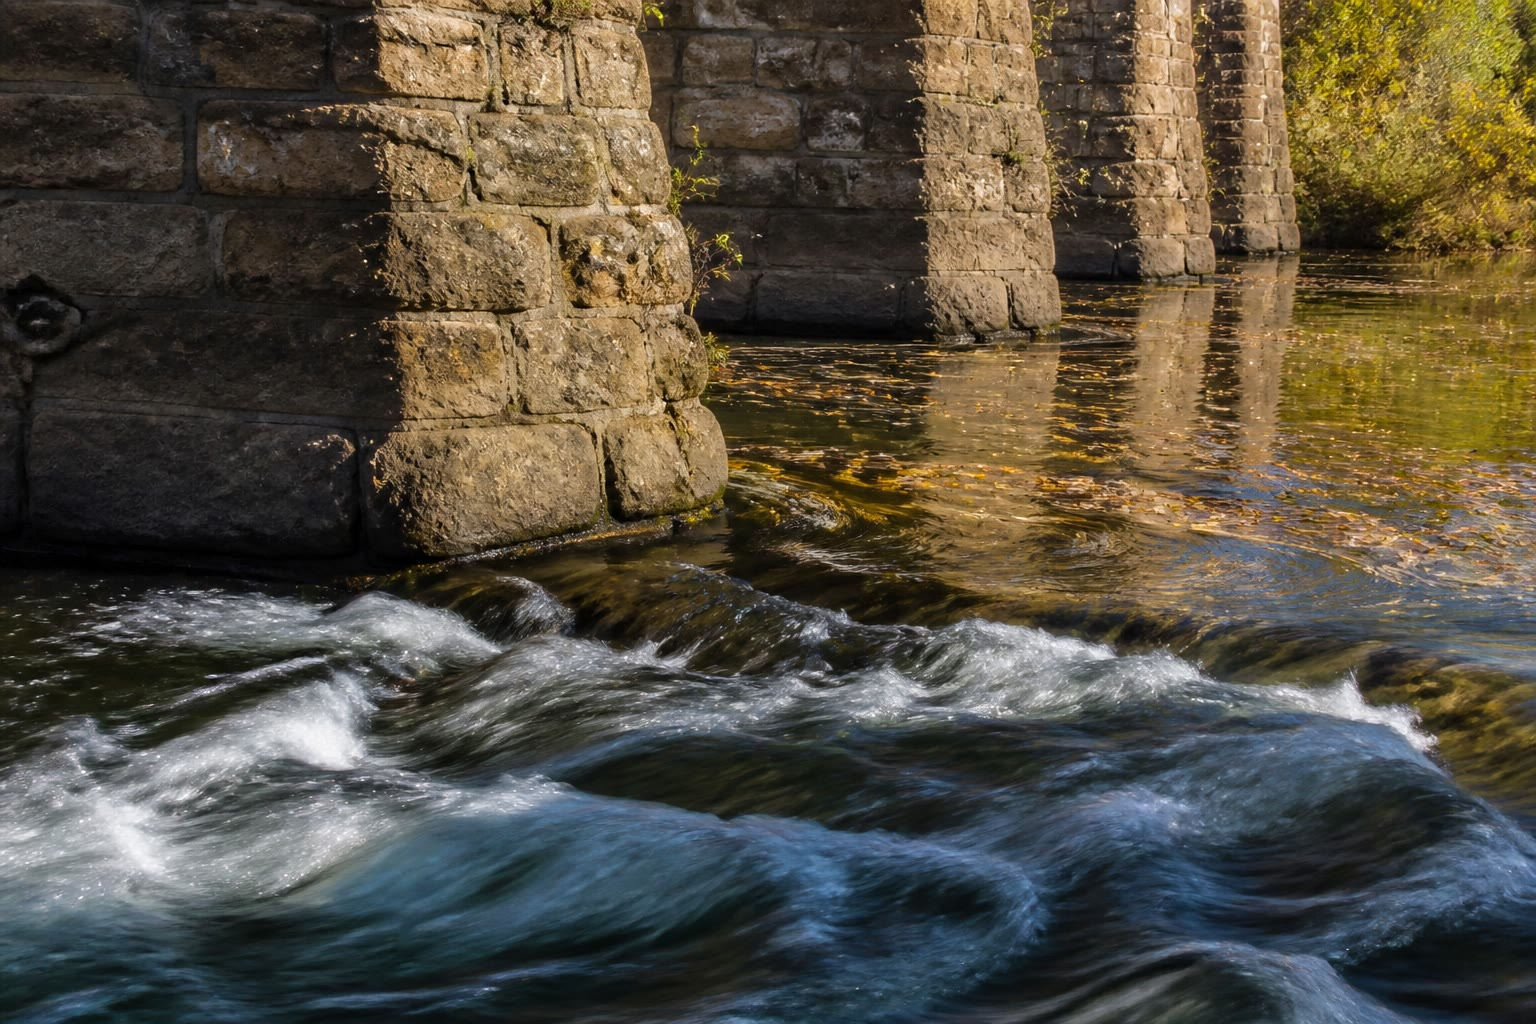
\includegraphics[width=0.58\linewidth]{images/book4/ai/b4-02-river-bridge-eddies.jpg}

{\small 河流流过桥梁：桥墩之间水流快而平稳，桥墩背风处有涡旋——需要在固定点读取的速度场，而非需要跟随的单一轨迹。}
\end{omfigure}


\section{连续介质描述}

\begin{definition}[流体质点；连续介质假设]\label{def:b2:fluid-kinematics:particle}
\index{流体质点}\index{连续介质假设}\index{介观尺度}
\emph{流体质点}是一小块流体，在流动尺度上足够小、可视为一点，
但又足够大，足以包含极大量的分子，
从而其密度 $\rho$、压强 $P$、
温度 $T$ 与平均速度 $\vect v$ 都是良定义的平均值
（\emph{介观}尺度，通常为一微米）。\emph{连续介质
假设}假定这样的尺度存在：分子的平均自由程 $\ell$
必须远小于流动的特征尺度 $L$，
即 $\ell/L \ll 1$。在大气压强下的空气中 $\ell \approx \qty{70}{nm}$；
在液体中 $\ell$ 即为分子大小。于是流体由
在每一点都有定义的\emph{场} $\rho(M, t)$、$P(M, t)$、$\vect v(M, t)$ 描述。
\end{definition}

\begin{definition}[拉格朗日描述与欧拉描述]\label{def:b2:fluid-kinematics:euler}
\index{拉格朗日描述}\index{欧拉描述}\index{流线}\index{迹线}\index{定常流动}
\emph{拉格朗日}描述跟踪每个流体质点：其
位置 $\vect r(t)$ 与速度 $\dd\vect r/\dd t$ 是
时间及其初始位置的函数。\emph{欧拉}描述给出
每个固定点 $M$、时刻 $t$ 处的速度 $\vect v(M, t)$，
即该时刻正经过 $M$ 的质点的速度。\emph{迹线}
是质点的轨迹；时刻 $t$ 的\emph{流线}是
在每一点都与 $\vect v(M, t)$ 相切的曲线；\emph{流管}是
由过一条闭合曲线的所有流线构成的曲面。若一个流动
的欧拉场不依赖于时间，则称其为\emph{定常的}（稳定的），
即 $\partial\vect v/\partial t = \vect 0$；此时流线与迹线
重合，且固定不变。
\end{definition}

\begin{example}[同一流动的两种描述]\label{ex:b2:fluid-kinematics:hose}
截面积为 $S$ 的花园水管中，水以体积流量 $Q$ 流动，其速度处处为 $v = Q/S$：
欧拉场是均匀的，
每个质点的拉格朗日运动也是匀速的。在渐缩喷管中，欧拉场仍是定常的，
但沿轴线 $v$ 增大：每个质点
\emph{加速}地通过，尽管任一固定点处的量都不随时间改变。
这正是
欧拉描述必须首先学会表达的内容。
\end{example}

\begin{omfigure}
\begin{tikzpicture}[font=\small, x=1cm, y=1cm, >=Stealth]
  \begin{scope}
    % streamlines of a converging channel
    \foreach \y in {-1.2,-0.6,0,0.6} {
      \draw[omDef, thick, postaction={decorate, decoration={markings, mark=at position 0.55 with {\arrow{>}}}}]
        (-2.8,\y) .. controls (-0.8,\y) and (0.2,{0.45*\y}) .. (2.8,{0.45*\y});
    }
    \draw[omDef, thick, postaction={decorate, decoration={markings, mark=at position 0.55 with {\arrow{>}}}}]
        (-2.8,1.2) .. controls (-0.8,1.2) and (0.2,0.54) .. (2.8,0.54)
        coordinate[pos=0.15] (P1) coordinate[pos=0.6] (P2) coordinate[pos=0.9] (P3);
    \draw[thick] (-2.8,1.6) .. controls (-0.8,1.6) and (0.2,0.75) .. (2.8,0.75);
    \draw[thick] (-2.8,-1.6) .. controls (-0.8,-1.6) and (0.2,-0.75) .. (2.8,-0.75);
    \fill[omThm] (P1) circle (2pt) node[above, font=\footnotesize, yshift=1pt] {$t_1$};
    \fill[omThm] (P2) circle (2pt) node[above, font=\footnotesize, yshift=1pt] {$t_2$};
    \fill[omThm] (P3) circle (2pt) node[above, font=\footnotesize, yshift=1pt] {$t_3$};
    \node[font=\footnotesize, align=center] at (0,-2.15) {定常流动：流线 $=$ 迹线，\\质点在管道变窄处加速};
  \end{scope}
  \begin{scope}[xshift=7.4cm]
    \draw[thick,->] (-2.8,-1.2) -- (2.8,-1.2) node[right, font=\footnotesize] {$x$};
    \draw[thick,->] (-2.8,-1.2) -- (-2.8,1.6);
    % velocity vectors at fixed points (Eulerian)
    \foreach \x in {-2.2,-1.2,-0.2,0.8,1.8} \foreach \y in {-0.6,0.2,1.0} {
      \draw[omDef, ->] (\x,\y) -- ({\x+0.5+0.12*\x},{\y+0.15*\y});
    }
    \node[omDef, font=\footnotesize] at (0,1.75) {欧拉描述：固定点处的 $\vect v(M,t)$};
    \draw[omThm, thick, ->] (-2.5,-0.9) .. controls (-1,-0.3) and (0.5,0.9) .. (2.4,1.3);
    \node[omThm, font=\footnotesize] at (2.2,0.7) {迹线};
    \node[font=\footnotesize, align=center] at (0,-1.95) {拉格朗日描述：跟随一个质点};
  \end{scope}
\end{tikzpicture}

{\small 左：定常的会聚流动——流线固定，
一个示踪质点沿其中一条流线运动，并随管道变窄而加速。
右：欧拉描述记录固定点处的速度矢量；
拉格朗日描述则沿其
迹线跟随该质点。}
\end{omfigure}

\section{随体导数}

\begin{theorem}[随体（质点）导数]\label{thm:b2:fluid-kinematics:material}
\index{随体导数}\index{对流加速度}
物理量 $G(M, t)$（标量或矢量）的
变化率，对经过 $M$ 点、在时刻 $t$ 的\emph{流体质点}而言，为
\[
\frac{\mathrm DG}{\mathrm Dt} = \frac{\partial G}{\partial t} + (\vect v\cdot
\operatorname{\vect{grad}})\,G ,
\qquad\text{特别地}\qquad
\vect a = \frac{\mathrm D\vect v}{\mathrm Dt} = \frac{\partial\vect v}{\partial t} +
(\vect v\cdot\operatorname{\vect{grad}})\,\vect v ,
\]
其中 $(\vect v\cdot\operatorname{\vect{grad}}) = v_x\partial_x + v_y\partial_y +
v_z\partial_z$。第一项是\emph{局域}变化率（即在固定点处），
第二项是\emph{对流}变化率（因为质点
会移向 $G$ 取值不同的位置）。对于速度，$(\vect v\cdot
\operatorname{\vect{grad}})\vect v = \operatorname{\vect{grad}}(v^2/2) +
(\operatorname{\vect{curl}}\vect v)\wedge\vect v$.
\end{theorem}

\begin{proof}
在 $\dd t$ 内质点由 $M$ 移至 $M + \vect v\,\dd t$，故 $\dd G =
G(M + \vect v\dd t, t + \dd t) - G(M, t) = \partial_tG\,\dd t + \dd t\,(v_x\partial_x
+ v_y\partial_y + v_z\partial_z)G$ 取到一阶（四变量函数的
链式法则）。矢量恒等式在 $x$
分量：$[\operatorname{\vect{grad}}(v^2/2)]_x = v_x\partial_xv_x + v_y\partial_x
v_y + v_z\partial_xv_z$ 和 $[(\operatorname{\vect{curl}}\vect v)\wedge\vect v]_x =
v_y(\partial_yv_x - \partial_xv_y) + v_z(\partial_zv_x - \partial_xv_z)$（其中
$\operatorname{\vect{curl}}\vect v$ 的各分量见
\cref{def:b2:fluid-kinematics:vorticity}）；其和为 $v_x\partial_xv_x +
v_y\partial_yv_x + v_z\partial_zv_x$。
\end{proof}

\begin{example}[稳定流动喷管中的加速度]\label{ex:b2:fluid-kinematics:nozzle}
沿喷管的一维稳定流动 $v(x) = v_0(1 + x/L)$：局域项
为零，且 $a = v\,\dd v/\dd x = v_0^2(1 + x/L)/L$。
质点以 $v_0 = \qty{2}{m/s}$ 进入，并以 $2v_0$ 离开，经过 $L
= \qty{5}{cm}$ 内，质点受 $a = 80$ 至 \qty{160}{m/s^2}，即八至十六倍 $g$，在
与时间无关的流动中。
\end{example}

\begin{example}[局域与对流]\label{ex:b2:fluid-kinematics:weather}
气象站处的温度在夜晚下降（$\partial T/
\partial t < 0$：局域），随风向北移动的空气团温度同样下降
（$\vect v\cdot\operatorname{\vect{grad}}T < 0$：对流，或
\emph{平流}）。装在随风漂移气球上的温度计
记录的是两项之和 $\mathrm DT/\mathrm Dt$；而气象站只
记录第一项。
\end{example}

\section{质量守恒}

\begin{definition}[质量流量与体积流量]\label{def:b2:fluid-kinematics:flowrate}
\index{质量流量}\index{体积流量}\index{质量通量}
通过有向曲面 $S$ 的\emph{质量流量}是单位时间内
穿过该面的质量，$D_m = \sum\rho\,\vect v\cdot\vect n\,\dd S$——
即\emph{质量流密度} $\vect j = \rho\vect v$ 的通量（单位
\unit{kg.m^{-2}.s^{-1}}）；\emph{体积流量}为 $D_V = \sum\vect v
\cdot\vect n\,\dd S$（\unit{m^3/s}）。若速度均匀且垂直于面积为
$S$ 的平面截面，则 $D_m = \rho vS$，$D_V = vS$。
\end{definition}

\begin{proof}
在 $\dd t$ 内穿过面元 $\dd S$ 的流体，即包含在
以 $\dd S$ 为底、$\vect v\,\dd t$ 为母线的斜柱体中，其
体积为 $\vect v\cdot\vect n\,\dd S\,\dd t$，质量则为该体积的 $\rho$ 倍。
\end{proof}

\begin{theorem}[质量的局域守恒]\label{thm:b2:fluid-kinematics:continuity}
\index{连续性方程}\index{散度}
流体中每一点处，
\[
\frac{\partial\rho}{\partial t} + \operatorname{div}(\rho\vect v) = 0 ,
\qquad\text{其中}\qquad
\operatorname{div}\vect A = \frac{\partial A_x}{\partial x} + \frac{\partial A_y}{\partial y} +
\frac{\partial A_z}{\partial z}
\]
为矢量场的\emph{散度}：即
$\vect A$ 穿过小体积表面的净外流通量（单位体积）。
等价地，$\mathrm D\rho/\mathrm Dt + \rho\operatorname{div}\vect v = 0$。
\end{theorem}

\begin{proof}
取固定小盒 $[x, x + \dd x]\times[y, y + \dd y]\times[z, z + \dd z]$。
其质量 $\rho\,\dd x\dd y\dd z$ 的变化率为 $\partial_t\rho\,\dd x\dd y
\dd z$。质量经 $x$ 处的面以 $j_x(x)\dd y\dd z$ 的速率流入，
并经 $x + \dd x$ 处的面以 $j_x(x + \dd x)\dd y\dd z$ 的速率流出：
净流出量为 $\partial_xj_x\,\dd x\dd y\dd z$，对 $y$ 和 $z$ 同理。
质量守恒——即质量不会凭空产生——给出 $\partial_t\rho = -
(\partial_xj_x + \partial_yj_y + \partial_zj_z)$。第二式由
$\operatorname{div}(\rho\vect v) = \vect v\cdot\operatorname{\vect{grad}}\rho +
\rho\operatorname{div}\vect v$.
\end{proof}

\begin{remark}[散度初识]\label{rem:b2:fluid-kinematics:divergence}
上述推导表明 $\operatorname{div}$ 度量的是离开
小盒的通量（单位体积）。将铺满有限
体积 $V$ 的诸小盒求和，内部面两两相消，只余
外表面：$\iint_{\partial V}\vect A\cdot\vect n\,\dd S = \iiint_V
\operatorname{div}\vect A\,\dd\tau$——即奥斯特罗格拉茨基
散度定理，将在\cref{ch:b2:maxwell-equations}中正式叙述，
并在电磁学中广泛应用；其证明见本科三年级
数学分册。对固定体积积分后，局域定律写作
$\dd m_V/\dd t = -D_m^{\text{外流}}$：体内质量的改变
即穿过边界的质量。
\end{remark}

\begin{omfigure}
\begin{tikzpicture}[font=\small, x=1cm, y=1cm, >=Stealth]
  \begin{scope}
    \draw[thick, fill=omDef!10] (0,0) rectangle (2.2,1.6);
    \draw[thick] (0,1.6) -- (0.6,2.1) -- (2.8,2.1) -- (2.2,1.6);
    \draw[thick] (2.2,0) -- (2.8,0.5) -- (2.8,2.1);
    \draw[omThm, very thick, ->] (-1.2,0.8) -- (-0.1,0.8) node[pos=0.3, above, font=\footnotesize] {$j_x(x)$};
    \draw[omThm, very thick, ->] (2.3,0.8) -- (3.6,0.8) node[pos=0.75, above, font=\footnotesize] {$j_x(x+\dd x)$};
    \node[font=\footnotesize] at (1.1,-0.35) {$\dd x$};
    \node[font=\footnotesize] at (-0.35,0.3) {$\dd y$};
    \node[font=\footnotesize] at (2.75,-0.05) {$\dd z$};
    \node[font=\footnotesize, align=left] at (1.3,-1.1) {$\partial_t\rho\,\dd\tau = -(\partial_x j_x + \partial_y j_y + \partial_z j_z)\,\dd\tau$};
  \end{scope}
  \begin{scope}[xshift=8.2cm]
    \draw[thick] (-2.4,1.1) .. controls (-1,1.1) and (0,0.5) .. (2.4,0.5);
    \draw[thick] (-2.4,-1.1) .. controls (-1,-1.1) and (0,-0.5) .. (2.4,-0.5);
    \draw[omDef, thick] (-2.4,0) ellipse (0.25 and 1.1);
    \draw[omDef, thick] (2.4,0) ellipse (0.12 and 0.5);
    \draw[omThm, very thick, ->] (-2.4,0) -- (-1.4,0) node[above, font=\footnotesize] {$v_1$};
    \draw[omThm, very thick, ->] (2.4,0) -- (3.6,0) node[above, font=\footnotesize] {$v_2$};
    \node[omDef, font=\footnotesize] at (-2.4,1.45) {$S_1$};
    \node[omDef, font=\footnotesize] at (2.4,0.85) {$S_2$};
    \node[font=\footnotesize] at (0,-1.6) {稳定：$\rho_1v_1S_1 = \rho_2v_2S_2$};
  \end{scope}
\end{tikzpicture}

{\small 左：固定箱体的质量守恒——经其六个面的净流出量，
每单位体积上的值，即为 $\rho\vect v$ 的散度。
右：稳定流动中，质量流量在流管的每一截面上
都相同。}
\end{omfigure}

\begin{corollary}[不可压缩流动；流管]\label{cor:b2:fluid-kinematics:incompressible}
\index{不可压缩流动}
若每个质点的密度保持不变，则称流动为\emph{不可压缩的}，
即 $\mathrm D\rho/\mathrm Dt = 0$，这等价于
\[
\operatorname{div}\vect v = 0 .
\]
均匀液体的流动是不可压缩的；速率远低于声速的气体亦然
（见\cref{ch:b2:sound-waves}）。稳定流动中，质量流量 $\rho vS$ 在
流管的每一截面上都相同；若流动还是不可压缩的，且 $\rho$ 均匀，
则 $vS$ 为常量，
即流体在管道变窄处加速。
\end{corollary}

\begin{proof}
$\mathrm D\rho/\mathrm Dt = -\rho\operatorname{div}\vect v$。对流管而言，
对两截面之间的体积应用积分形式的守恒关系：
侧表面无通量（速度与之相切），处于稳态，
因此流入量等于流出量。
\end{proof}

\begin{example}[血液]\label{ex:b2:fluid-kinematics:blood}
主动脉（截面积 \qty{2.5}{cm^2}）输送 \qty{5}{L/min} $= \qty{83}{cm^3/s}$：
其速率为 $v = \qty{33}{cm/s}$。同样的流量通过约 $10^{10}$
根毛细血管，总截面积约为 \qty{2500}{cm^2}：$v = \qty{0.3}{mm/s}$——
足够慢，以便物质透过管壁交换，这正是分支的意义所在。
\end{example}

\section{涡量与无旋流动}

\begin{definition}[涡量]\label{def:b2:fluid-kinematics:vorticity}
\index{涡量}\index{旋度}\index{无旋流动}
流动的\emph{涡量}是矢量场
\[
\vect\omega = \operatorname{\vect{curl}}\vect v , \qquad
\operatorname{\vect{curl}}\vect A = \Bigl(\frac{\partial A_z}{\partial y} -
\frac{\partial A_y}{\partial z},\; \frac{\partial A_x}{\partial z} - \frac{\partial A_z}
{\partial x},\; \frac{\partial A_y}{\partial x} - \frac{\partial A_x}{\partial y}\Bigr) .
\]
在 $\vect\omega = \vect 0$ 的区域，流动称为\emph{无旋的}。
\end{definition}

\begin{proposition}[涡量度量局部转动]\label{prop:b2:fluid-kinematics:rotation}
以 $M$ 为中心的一个小流体微团，整体上
以角速度 $\vect\Omega = \tfrac12\vect\omega(M)$ 转动。在刚体式
转动 $\vect v = \vect\Omega\wedge\vect{OM}$ 中，涡量处处均匀，
$\vect\omega = 2\vect\Omega$；在平面剪切流 $\vect v = ky\,\vect e_x$
中，涡量为 $\vect\omega = -k\vect e_z$：放入剪切流中的桨轮会转动，
尽管流线是直线。
\end{proposition}

\begin{proof}
在 $M$ 附近，$\vect v(M + \vect\epsilon) = \vect v(M) + \mathbf G\vect\epsilon$，其中
$\mathbf G$ 为 $\partial_jv_i$ 构成的矩阵；将其分解为对称部分
（纯应变，它使微团伸展而不整体转动），与反对称部分
其矩阵 $\tfrac12(\partial_jv_i -
\partial_iv_j)$ 与映射 $\vect\epsilon \mapsto \tfrac12\vect\omega\wedge\vect\epsilon$ 的矩阵相同
（见\cref{thm:b2:rigid-body-mechanics:field}）。绕 $\vect e_z$ 轴的刚体转动：
$\vect v = \Omega(-y, x, 0)$, $\omega_z = \partial_xv_y - \partial_yv_x = 2\Omega$.
剪切：$\omega_z = -\partial_y(ky) = -k$。
\end{proof}

\begin{definition}[速度势；环量]\label{def:b2:fluid-kinematics:potential}
\index{速度势}\index{环量（速度的）}\index{势流}
在无旋流动中，速度由\emph{速度
势}导出：$\vect v = \operatorname{\vect{grad}}\varphi$（$\vect v$ 沿路径的环量
则只依赖于端点，$\int_A^B\vect v
\cdot\dd\vect l = \varphi(B) - \varphi(A)$）。若流动同时不可压缩，
则 $\Delta\varphi = \operatorname{div}\operatorname{\vect{grad}}
\varphi = 0$：势函数满足拉普拉斯方程，与无电荷区域中的
静电势完全相同——这种流动称为\emph{势流}。
速度沿闭合曲线 $C$ 的\emph{环量}
为 $\Gamma = \oint_C\vect v\cdot\dd\vect l$。
\end{definition}

\begin{proof}
单连通区域上无旋的场为梯度场，以及
梯度场无旋（$\partial_y\partial_z\varphi = \partial_z\partial_y\varphi$），
这些属于本科二年级数学分册的内容；拉普拉斯方程由
$\operatorname{div}\vect v = 0$ 推出。
\end{proof}

\begin{example}[三种平面流动]\label{ex:b2:fluid-kinematics:planeflows}
\index{滞止流}\index{点涡}\index{兰金涡}
(i) \emph{滞止流} $\vect v = k(x, -y)$：$\operatorname{div}\vect v =
0$，$\vect\omega = \vect 0$，$\varphi = \tfrac12k(x^2 - y^2)$；流线
$xy = $ 常数，为双曲线——射流撞击壁面、在轴线附近的情形。(ii)
\emph{点涡} $\vect v = \dfrac{\Gamma}{2\pi r}\vect e_\theta$（平面
极坐标）：流动不可压缩，且\emph{除 $r = 0$ 外处处无旋}
，$\varphi = \Gamma\theta/2\pi$（多值），并且绕中心任一圆周的
环量均为 $\Gamma$——涡量
集中在轴线上。(iii) \emph{兰金涡}：半径
$r < a$ 的核心区做刚体式转动 $v_\theta = \Omega r$（涡量为 $2\Omega$），
在外部与点涡 $v_\theta = \Omega a^2/r$ 相衔接，它是
龙卷风、浴缸漩涡或桥墩后涡旋的模型——
速率在核心边缘处达到峰值。
\end{example}

\begin{omfigure}
\begin{tikzpicture}[font=\small, x=1cm, y=1cm, >=Stealth]
  \begin{scope}
    \foreach \c in {0.3,0.8,1.6,2.8} {
      \draw[omDef, thick, domain={\c/2.4}:2.4, samples=40, postaction={decorate, decoration={markings, mark=at position 0.5 with {\arrow{>}}}}] plot (\x,{\c/\x});
      \draw[omDef, thick, domain=-2.4:{-\c/2.4}, samples=40, postaction={decorate, decoration={markings, mark=at position 0.5 with {\arrow{<}}}}] plot (\x,{-\c/\x});
    }
    \draw[thick] (-2.5,0) -- (2.5,0);
    \draw[->] (0,0) -- (0,2.6) node[right, font=\footnotesize] {$y$};
    \node[font=\footnotesize] at (0,-0.4) {滞止流 $\vect v = k(x,-y)$};
  \end{scope}
  \begin{scope}[xshift=6.6cm]
    \foreach \r in {0.5,0.9,1.3,1.7} \draw[omDef, thick, postaction={decorate, decoration={markings, mark=at position 0.25 with {\arrow{>}}}}] (0,0) circle (\r);
    \fill (0,0) circle (1.5pt);
    \node[font=\footnotesize] at (0,-2.2) {点涡 $v_\theta = \Gamma/2\pi r$};
  \end{scope}
  \begin{scope}[xshift=10.6cm]
    \begin{axis}[omaxis, axis x line=bottom, axis y line=left, width=4.4cm, height=3.9cm, at={(0,-1.9cm)},
        xlabel={$r/a$}, ylabel={$v_\theta$}, xmin=0, xmax=4, ymin=0, ymax=1.2, xtick={1,2,3}, ytick=\empty,
        xlabel style={at={(axis description cs:0.5,-0.12)}, anchor=north},
        ylabel style={at={(axis description cs:-0.08,0.5)}, rotate=90, anchor=south}, samples=60]
      \addplot[omThm, thick, domain=0:1] {x};
      \addplot[omThm, thick, domain=1:4] {1/x};
      \node[font=\scriptsize] at (axis cs:0.55,0.85) {$\Omega r$};
      \node[font=\scriptsize] at (axis cs:2.6,0.62) {$\Omega a^2/r$};
    \end{axis}
  \end{scope}
\end{tikzpicture}

{\small 三种平面流动。左：滞止流动，无旋，
流线呈双曲线形。中：点涡——圆形
流线，但远离中心处涡量为零。右：
兰金涡的速度分布，核心区为刚体转动，
外部为点涡。}
\end{omfigure}

\begin{remark}[为何环量重要]\label{rem:b2:fluid-kinematics:stokes}
对面积为 $\dd S$、法向为 $\vect n$ 的小平面回路，
环量为 $\oint\vect v\cdot\dd\vect l = \vect\omega\cdot\vect n\,\dd S$——
涡量即单位面积上的环量，正如
散度即单位体积上的通量。（以刚体转动为例验证：
$2\pi r\cdot\Omega r = 2\Omega\cdot\pi r^2$）。对曲面求和，
即得斯托克斯定理 $\oint_C\vect v\cdot\dd\vect l = \iint_S
\operatorname{\vect{curl}}\vect v\cdot\vect n\,\dd S$，其表述见
\cref{ch:b2:maxwell-equations}。机翼靠
绕自身的环量产生升力；涡线在理想流体中
持续存在（开尔文定理）——这正是桥墩身后的涡旋
能持续如此之久的原因。
\end{remark}

\begin{method}[读取速度场]\label{met:b2:fluid-kinematics:reading}
给定 $\vect v(M, t)$：（1）是否为稳定流动？（$\partial_t\vect v = \vect 0$）；（2）
是否不可压缩？（$\operatorname{div}\vect v = 0$）；（3）是否
无旋？（$\operatorname{\vect{curl}}\vect v = \vect 0$；若是，则求
$\varphi$）；（4）求流线：由 $\dd x/v_x = \dd y/v_y = \dd z/
v_z$ 在固定 $t$ 时确定，并求迹线：由 $\dd\vect r/\dd t = \vect v(\vect r,
t)$；（5）计算加速度 $\partial_t\vect v + (\vect v\cdot
\operatorname{\vect{grad}})\vect v$。在平面极坐标 $(r, \theta)$ 下，
$\operatorname{div}\vect v = \dfrac1r\dfrac{\partial(rv_r)}{\partial r} + \dfrac1r
\dfrac{\partial v_\theta}{\partial\theta}$ 且 $\omega_z = \dfrac1r\dfrac{\partial(rv_\theta)}
{\partial r} - \dfrac1r\dfrac{\partial v_r}{\partial\theta}$（在本阶段不加证明地承认；推导见
\cref{ch:b2:maxwell-equations}）。
\end{method}

\section{练习}

\begin{exercise}[$\star$]\label{exo:b2:fluid-kinematics:1}
空气的平均自由程在 \qty{1}{bar} 时为 \qty{70}{nm}，并随
$1/P$ 成正比变化。判断连续介质描述在下列情形中是否成立：（a）汽车周围的空气，
（b）\qty{1}{bar} 下，位于 \qty{1}{\micro m} 微通道内的空气，（c）
\qty{100}{km} 高空（$P \approx \qty{3e-7}{bar}$）处绕
\qty{1}{m} 卫星飞行的空气？并给出各情形下的 $\ell/L$。
\end{exercise}

\begin{exercise}[$\star$]\label{exo:b2:fluid-kinematics:2}
一维稳定流动 $v(x) = v_0(1 + x/L)$，$0 \le x \le L$。
求位于 $x$ 处质点的加速度；求其从 $0$ 运动到
$L$ 所需的时间，并与 $L/v_0$ 和 $L/2v_0$ 比较。
\end{exercise}

\begin{exercise}[$\star$]\label{exo:b2:fluid-kinematics:3}
半径为 $R$ 的管道中，速度分布为 $v(r) = v_{\max}(1 -
r^2/R^2)$，沿轴线方向。求体积流量与平均速率 $\langle v\rangle
= D_V/\pi R^2$，并算出 $R = \qty{5}{mm}$、$v_{\max} = \qty{0.4}{m/s}$ 时的数值。
\end{exercise}

\begin{exercise}[$\star$]\label{exo:b2:fluid-kinematics:4}
对每个速度场，判断流动是否不可压缩以及是否
无旋；给出涡量：（a）$\vect v = (ax, -ay, 0)$；（b）
$\vect v = (-\Omega y, \Omega x, 0)$；（c）$\vect v = (ax, ay, 0)$；（d）$\vect v =
(ky, 0, 0)$；（e）$\vect v = (ax, -ay, bz)$——对于何值的 $b$，该流动
是不可压缩的？
\end{exercise}

\begin{exercise}[$\star\star$]\label{exo:b2:fluid-kinematics:5}
一根内径为 \qty{12}{mm} 的园艺水管，
可在 \qty{50}{s} 内注满一只 \qty{10}{L} 的水桶。求水管中的速率，以及 \qty{3}{mm} 喷管中的速率；若
喷管在 \qty{4}{cm} 内渐缩，估算穿过它的质点的平均加速度
（以 $g$ 为单位）；求质点在喷管中所用的时间。
\end{exercise}

\begin{exercise}[$\star\star$]\label{exo:b2:fluid-kinematics:6}
非稳定平面流动 $\vect v = (U, V\cos\omega t)$，其中 $U$、$V$、$\omega$
均为常量。（a）求时刻 $t$ 的流线；（b）求
$t = 0$ 时位于原点的质点的迹线。（c）当 $V = U$ 时，画出 $t = 0$ 与
$t = \pi/2\omega$ 两个时刻的草图，并说明二者为何不同；（d）求质点的加速度。
\end{exercise}

\begin{exercise}[$\star\star$]\label{exo:b2:fluid-kinematics:7}
一条宽 \qty{50}{m}、深 \qty{2.0}{m} 的河流，流速为 \qty{1.2}{m/s}。（a）
求流量。（b）河流进入一段宽 \qty{15}{m}、深 \qty{4.0}{m} 的峡谷，求其中
的速率。（c）一条支流汇入，增加 \qty{30}{m^3/s} 的流量；下游河宽
\qty{60}{m}、深 \qty{2.5}{m}，求其速率。（d）热气体稳定地流过
等截面管道，两点之间的温度
在压强不变时加倍，其速率如何变化？
\end{exercise}

\begin{exercise}[$\star\star$]\label{exo:b2:fluid-kinematics:8}
\emph{兰金涡。}$v_\theta = \Omega r$，当 $r < a$ 时；$v_\theta = \Omega a^2/r$
当 $r > a$ 时。（a）求各区域中的涡量（用极坐标公式）；（b）
求以轴线为圆心、半径为 $r$ 的圆周上的环量，在两个
区域中分别计算，并与涡量通量相联系。（c）龙卷风：$a = \qty{50}{m}$，
$v_{\max} = \qty{70}{m/s}$，求 $\Omega$、$\Gamma$，以及 \qty{500}{m} 处的速率。
（d）核心区的流动是否无旋？外部呢？“旋转”
在物理上位于何处？
\end{exercise}

\begin{exercise}[$\star\star$]\label{exo:b2:fluid-kinematics:9}
\emph{滞止流动} $\vect v = k(x, -y)$。（a）求速度势 $\varphi$，并
验证 $\Delta\varphi = 0$。（b）求流线；函数 $\psi = kxy$ 在
流线上为常数——证明 $v_x = \partial\psi/\partial y$，$v_y = -\partial\psi/
\partial x$（即\emph{流函数}）。（c）求加速度场，并证明它
是 $\operatorname{\vect{grad}}(v^2/2)$，并加以解释。（d）求
从 $(x_0, y_0)$ 出发的质点的迹线，已知 $x = x_0\eu^{kt}$，$y = y_0\eu^{-kt}$。
\end{exercise}

\begin{exercise}[$\star\star\star$]\label{exo:b2:fluid-kinematics:10}
\emph{膨胀流动。}一维流动 $v(x, t) = x/(t + \tau)$
其中 $t > 0$，$\tau > 0$ 为常量。（a）求迹线，并证明 $x(t) = x_0(1 +
t/\tau)$；求质点的加速度，既可由迹线，也可由
随体导数求得。（b）各时刻密度均匀，
记为 $\rho(t)$，利用质量守恒求 $\rho(t)$。（c）通过
考察两质点之间的质量加以检验。（d）为何该场可以作为
均匀膨胀宇宙的一维模型？
\end{exercise}

\begin{exercise}[$\star\star\star$]\label{exo:b2:fluid-kinematics:11}
\emph{水流中的源。}叠加均匀流 $\vect v = U\vect e_x$
与平面源 $\vect v = \dfrac{q}{2\pi r}\vect e_r$（$q$ 为沿 $z$ 方向单位长度的
体积流量）。（a）求势函数 $\varphi = Ux +
(q/2\pi)\ln r$；验证两种流动均不可压缩且无旋
（原点除外）。（b）求驻点。（c）求流函数 $\psi
= Uy + q\theta/2\pi$；过驻点的流线为
$r\sin\theta = (q/2\pi U)(\pi - \theta)$：画出该流线示意图。（d）证明在远下游
该流线位于 $y = \pm q/2U$ 处：该流线外侧的流动
即为宽度为 $q/U$ 的钝头半体绕流。
\end{exercise}

\begin{exercise}[$\star\star\star$]\label{exo:b2:fluid-kinematics:12}
\emph{涡旋与汇。}平面流动 $\vect v = -\dfrac{q}{2\pi r}\vect e_r +
\dfrac{\Gamma}{2\pi r}\vect e_\theta$，其中 $r > a$。（a）证明它
不可压缩且无旋。（b）求流线：对数螺线
$r = r_0\eu^{-q\theta/\Gamma}$。（c）求质点的加速度：证明它
为纯径向的，$-v^2/r\,\vect e_r$。（d）求质点螺旋运动
从 $r_0$ 到 $a$ 所需的时间，以及其绕行的圈数。（e）数值：$q =
\qty{1.5e-3}{m^2/s}$，$\Gamma = \qty{3e-2}{m^2/s}$，$r_0 = \qty{0.5}{m}$，
$a = \qty{2}{cm}$。
\end{exercise}

\section{问题：从排水口到飓风}

\begin{problem}[{周末问题——三种尺度上的同一运动学：
排水口上方的漩涡、龙卷风，以及从卫星上看到的气旋}]
\label{pb:b2:fluid-kinematics:1}

\medskip
\noindent\textbf{第一部分——浴缸。}
浴缸经半径 $a = \qty{2}{cm}$ 的孔排水，
水深 $h = \qty{20}{cm}$，以体积流量 $D_V =
\qty{0.30}{L/s}$ 流出。远离孔口时，流动可视为平面流动
（与深度无关）：$\vect v = v_r(r)\vect e_r + v_\theta(r)\vect e_\theta$。
\begin{enumerate}
  \item 利用通过半径为 $r$ 的圆柱面的质量守恒，
        （圆柱面高为 $h$），证明 $v_r = -q/2\pi r$，其中 $q = D_V/h$；
        求 $q$ 的数值。
  \item 拔塞之前，水曾被搅动，
        并在 $r = \qty{50}{cm}$ 处具有 \qty{1.0}{cm/s} 的转动速度。假设
        每一圈水在向内运动过程中保持其角动量不变
        （$rv_\theta$ 为常量），求 $v_\theta(r)$ 及
        环量 $\Gamma$。
  \item 验证该流动在
        $r > a$ 时不可压缩且无旋。
  \item 流线：证明它们为对数螺线，并求
        质点从 $r = \qty{50}{cm}$ 运动到
        $r = a$ 时绕行的圈数。
  \item 求质点从 \qty{50}{cm} 运动到排水孔所需的时间，以及
        到达时的方位速率。
  \item 求 $r$ 处质点的加速度，并与 $g$ 比较（$r = a$ 处）。
        （自由面在压强须与之平衡处下凹——
        即漏斗；见下一章。）
  \item 地球自转使浴缸中静止的任一流体获得一个
        “背景”转动，其局地竖直方向的转动速率为
        $\Omega_\oplus\sin\lambda \approx \qty{5e-5}{rad/s}$。比较它在
        \qty{50}{cm} 处给出的方位速率与搅动产生的
        \qty{1}{cm/s}，并说明排水浴缸的转向
        是否由半球决定。
\end{enumerate}

\medskip
\noindent\textbf{第二部分——作为兰金涡的龙卷风。}
核心半径 $a = \qty{60}{m}$，最大风速 $v_{\max} = \qty{80}{m/s}$，空气
密度 $\rho = \qty{1.2}{kg/m^3}$。
\begin{enumerate}[resume]
  \item 写出两个区域中的 $v_\theta(r)$，并给出 $\Omega$ 与 $\Gamma$。
  \item 求核心内外的涡量；画出 $v_\theta$ 与 $\omega_z$
        随 $r$ 变化的示意图。
  \item 求核心边缘处空气质点的加速度，
        并与 $g$ 比较。
  \item 证明置于核心外部的小桨轮绕龙卷风漂移，
        而其自身不绕自轴旋转；
        置于核心内部的桨轮则每绕轴旋转一周，
        自身也转动一圈。
  \item 求核心每米高度的动能。
  \item 求外部流动每米高度的动能，
        范围为 $a$ 至 $R = \qty{5}{km}$；
        为何它仅对 $R$ 呈对数依赖？
  \item 若高度为 \qty{1}{km}，求总动能，并与
        \qty{1}{t} TNT 释放的能量（\qty{4.2}{GJ}）作比较。
  \item 龙卷风中空气也会向内、向上流动。若核心
        由其侧面以 \qty{5}{m/s} 的径向流入补给，
        该流入层的高度为最初 \qty{300}{m}，求
        该层顶部空气须达到的竖直速率（在
        核心截面上均匀分布）？
\end{enumerate}

\medskip
\noindent\textbf{第三部分——气旋。}
热带气旋可视为核心半径为
$a = \qty{40}{km}$、$v_{\max} = \qty{50}{m/s}$ 的兰金涡。地球自转
通过\emph{行星涡量}$f = 2\Omega_\oplus\sin\lambda
\approx \qty{5e-5}{s^{-1}}$，在纬度 \qty{20}{\degree} 处：相对地面
静止的一圈空气在惯性参考系中已具有
绕任一竖直轴的方位速率 $fr/2$。
\begin{enumerate}[resume]
  \item 求气旋核心的涡量及其环量 $\Gamma$；
        将核心涡量与 $f$ 作比较。
  \item 半径为 $r_0 = \qty{500}{km}$ 的一圈空气，最初相对地面静止，
        在低压作用下被吸向中心。假设其
        关于轴的单位质量角动量 $r(v_\theta + fr/2)$ 守恒，
        求其相对地面的速度
        $v_\theta$ 在 $r = \qty{100}{km}$ 处与
        $r = \qty{40}{km}$ 处的值。
  \item 北半球中气旋沿哪个方向旋转，
        为何如此？为何气旋的转向是确定的，
        而浴缸则不然？
  \item 为何空气不能经此方式一直被吸至轴线——
        是什么限制了风速并形成台风眼？
  \item 空气以 \qty{5}{m/s} 的速度，经
        半径为 \qty{500}{km}、高为 \qty{1}{km} 的圆柱面汇入气旋：求
        被吸入的质量流量（$\rho = \qty{1.2}{kg/m^3}$）。
  \item 气旋整体以 \qty{6}{m/s} 的速度向西移动。
        试用涡旋在其自身参考系中的场 $\vect v_0$ 表示
        从地面所见的欧拉速度场；该流动在地面参考系中
        是否定常？风暴的哪一侧
        风更强？
\end{enumerate}

\medskip
\noindent\textbf{第四部分——流量与总结。}
\begin{enumerate}[resume]
  \item 雨以 \qty{50}{mm/h} 的速率降落在 \qty{10}{km^2} 的集水区上，
        且全部汇入截面积为 \qty{40}{m^2} 的河流：求
        洪水期河流的平均流速。
  \item 血液：主动脉（\qty{2.5}{cm^2}）输送 \qty{5.0}{L/min}；
        毛细血管的总截面积为 \qty{0.25}{m^2}：求各处的流速；
        并求血液流过一根 \qty{1}{mm} 长的毛细血管所需的时间。
  \item 截面积为 $S$ 的水箱经截面积为 $s$ 的孔在
        底部排水，出口速率为 $\sqrt{2gh}$（$h$ 为水位
——此为承认的结果，将在下一章推导）。写出
        质量守恒，并求 $h(t)$ 及排空时间，
        取 $S = \qty{1}{m^2}$，$s = \qty{1}{cm^2}$，$h_0 = \qty{1}{m}$。
  \item 将第一至第三部分的三种流动列于一张表中：
        半径、速率、核心涡量、环量——以及
        在内流过程中守恒的量，正是使它们
        旋转加快的量。
\end{enumerate}
\end{problem}
